\documentclass{cpepaper}
\usepackage{amsmath, amssymb}

\title{การจำแนกกลุ่มของสัญญาณโจมตีแบบจำลองการเรียนรู้เชิงลึก}
\author{\IEEEauthorblockN{ศิระกร ลำใย\IEEEauthorrefmark{1},
วัชรพัฐ เมตตานันท\IEEEauthorrefmark{2}, และ 
จิตร์ทัศน์ ฝักเจริญผล\IEEEauthorrefmark{3}}
\IEEEauthorblockA{ภาควิชาวิศวกรรมคอมพิวเตอร์ คณะวิศวกรรมศาสตร์ มหาวิทยาลัยเกษตรศาสตร์\\
Email: \IEEEauthorrefmark{1}sirakorn.l@ku.th,
\IEEEauthorrefmark{2}vacharapat@eng.src.ku.ac.th,
\IEEEauthorrefmark{3}jtf@ku.ac.th}}

\begin{document}
\maketitle
\section*{บทคัดย่อ}
บทความวิชาการนี้กล่าวถึงการฝึกสอนแบบจำลองอย่างง่ายเพื่อค้นหารูปแบบของสัญญาณรบกวนที่สามารถโจมตีชุดข้อมูลรับเข้าให้ได้ผลลัพธ์ของแบบจำลองที่ผิดเพี้ยนไปได้ โดยพิจารณาการโจมตีบนโครงข่ายประสาทเทียมแบบเชื่อมถึงกันทั่ว และโครงข่ายประสาทเทียมแบบสังวัฒนาการ โครงข่ายประสาทเทียมทั้งสองแบบถูกฝึกสอนด้วยชุดข้อมูล MNIST ซึ่งมีชุดข้อมูลสำหรับฝึกสอนจำนวน 60,000 จุด หลังจากการฝึกสอนโครงข่ายประสาทเทียม นำข้อมูลทดสอบจำนวน 10,000 จุด มาทำการหาสัญญาณโจมตีความยาวเท่าจำนวนจุดทดสอบ และพยายามทำการเรียนรู้จัดหมวดหมู่ ผลลัพธ์ที่ได้คือ\dots
\vskip 12pt
\noindent คำสำคัญ: ปัญญาประดิษฐ์, จักรกลเรียนรู้, การเรียนรู้เชิงลึก, การโจมตีการเรียนรู้
\section*{Abstract}
blablabla
\vskip 12pt
\noindent Keywords: Artificial Intelligence, Machine Learning, Deep Learning, Adversarial Attack

\section{ความสำคัญและที่มา}
แบบจำลองจักรกลเรียนรู้ (machine learning models) นั้นถูกใช้อย่างกว้างขวางในปัจจุบัน อย่างไรก็ตามแบบจำลองใดๆ นั้นอาจมีความผิดพลาดต่อการทำการโจมตีประสงค์ร้าย (adversarial attacks) เพื่อจงใจให้ผลลัพธ์ที่แบบจำลองนั้นคาดเดามีความผิดพลาดจากผลลัพธ์ที่ควรจะเป็น

ในการเรียนรู้เชิงตัวแปรเสริม (parameter-based learning) นั้น ตัวแปรเสริม (parameters) ค่าน้ำหนัก (weights) บนแบบจำลองการเรียนรู้เชิงลึก (deep learning models) เป็นตัวกำหนดความฉลาดของแบบจำลอง อาจมีตัวแปรเสริมบางชุดที่ทำให้แบบจำลองมีช่องโหว่ต่อการโจมตีประสงค์ร้าย การโจมตีนั้นอาจเกิดจากการเพิ่มสัญญาณรบกวนซึ่งผ่านการคำนวน (calculated artefacts) เข้าสู่ข้อมูลรับเข้า (inputs) ซึ่งทำให้ความผิดพลาดของแบบจำลองในการพยากรณ์คำตอบนั้นเปลี่ยนไปอย่างชัดเจน

\section{ชุดวรรณกรรมและกระบวนวิธี}

\subsection{การโจมตีการเรียนรู้}

เราจะกล่าวถึงแบบจำลองที่ถูกฝึกสอนให้จัดจำแนกข้อมูลชุด $X$ และ $Y$ และพิจารณาข้อมูลรับเข้า $(x, y)$ หนึ่งจุดบนชุดทดสอบ จะนิยามข้อมูลโจมตี (adversarial) $\tilde{x}$ ว่า
\begin{equation}
    \tilde{x} = x + \eta
\end{equation}
เมื่อเรียก $\eta$ ว่าสัญญาณรบกวน (perturbations)

ข้อสังเกตที่เกิดขึ้นคือเราอาจะนิยามชุดสัญญาณรบกวนดังกล่าว ว่ามีความเข้มข้น (intensity) ในระดับที่ต่ำกว่าตามนุษย์จะมองเห็น กล่าวคือเมื่อเทียบกับชุดข้อมูลรับเข้าแล้ว ช่วง (range) ของสัญญาณรบกวนนั้นน้อยกว่าช่วงของข้อมูลรับเข้าที่เป็นไปได้มาก การนิยามดังกล่าวจะใช้การนิยามเซตของสัญญาณรบกวนที่เป็นไปได้ทั้งหมด (พิจารณาว่ามีค่า $\eta$ ที่เป็นไปได้หลายค่า และแต่ละค่าโจมตีแบบจำลองได้แตกต่างกันออกไป) ว่า
\begin{equation}
    H = \{ \eta: \|\eta\|_\infty \leq \epsilon\}
    \label{perturbation-set}
\end{equation}
เมื่อนิยามให้ตัวดำเนินการนอร์มอนันต์ (infinity norm) เป็น
\begin{equation}
    \|x\|_\infty = \max_i{x_i}
\end{equation}
และค่า $\epsilon$ เป็นค่าคงที่บ่งบอกความเข้มข้นของสัญญาณมากสุดที่รับได้ โดยมากมักมีค่าน้อย

\subsection{ฟังก์ชันสูญเสีย และการฝึกสอนแบบจำลองด้วยวิธีก้าวเคลื่อนถอยหลัง}
พิจารณาการเรียนรู้แบบจำลอง $M$ จะพบว่าการหาตัวแปรเสริม (parameters) $\theta$ ที่ดีที่สุดของ $M$ นั้นทำได้ด้วยการนิยามฟังก์ชันสูญเสีย (loss function) $\ell_i $ของจุดฝึกหัด (training point) $i$ ได้ โดยให้ฟังก์ชันสูญเสียเป็นฟังก์ชันที่เปรียบเทียบเป้าหมาย (target) $y_i$ จากชุดฝึกหัด และคำตอบ $\hat{y}_i = M(x_i)$ จากชุดคุณสมบัติ (features) $x_i$ ที่ถูกป้อนเข้าแบบจำลอง

เราอาจนิยามฟังก์ชันสูญเสียอย่างง่ายได้เป็นฟังก์ชันผลของผลต่างกำลังสอง
\begin{equation}
    \ell_i = \sum_{i=1}^{M}{(\hat{y}_i - y_i)^2} = \sum_{i=1}^{M}{(M(x_i) - y_i)^2}
    \label{mse-loss}
\end{equation}
เมื่อ $M$ เป็นขนาดของเป้าหมาย (target) สังเกดว่ายิ่งค่าของ $\hat{y}_i$ และ $y_i$ ต่างกันมากเท่าใด (มองอีกมุมหนึ่ง คือยิ่งตอบผิดมากเท่าใด) ค่าดังกล่าวก็จะยิ่งเพิ่มขึ้นมากเท่านั้น อย่างไรก็ดี ในการฝึกสอนแบบจำลองการเรียนรู้เชิงการจำแนก (classification) ส่วนมาก มักใช้ฟังก์ชันสูญเสียเป็นฟังก์ชันสูญเสียแบบความวุ่นวายข้ามชั้น (cross entropy loss)
\begin{equation}
    \ell_i = -\sum_{c=1}^{M}y_{o,c}\ln(p_{o,c})
    \label{cross-entropy-loss}
\end{equation}
เมื่อ $M$ เป็นจำนวนชั้น (class) ที่เป็นไปได้ $y$ เป็นค่าฐานสองที่บ่งบอกว่าชั้นข้อมูล (class) $c$ เป็นคำตอบที่ถูกต้องสำหรับการคาดเดา (observation) $o$ และ $p$ เป็นค่าความน่าจะเป็นที่การคาดเดา $o$ ตอบว่าเป็นชั้นข้อมูล $c$

นอกจากนี้เราอาจนิยามผลรวมของฟังก์ชันสูญเสียทั่วทั้งชุดฝึกสอน
\begin{equation}
    \mathcal{L} = \sum_{i=1}^{N}{l_i}
    \label{total-loss}
\end{equation}
เป็นผลรวมของฟังก์ชันสูญเสียบนทุกจุดฝึกหัด เมื่อ $N$ เป็นขนาดของชุดฝึกหัด (training set)

อย่างไรก็ดี แม้สมการ \ref{mse-loss} และ \ref{cross-entropy-loss} จะดูเหมือนพิจารณาค่าสูญเสียที่เปลี่ยนไปเมื่อชุดของข้อมูลฝึกหัดเปลี่ยน แต่พึงระวังว่าการนิยามฟังก์ชันสูญเสียดังกล่าว มีขึ้นเพื่อทดสอบว่าค่าตัวแปรเสริม $\theta$ ใดๆ ส่งผลให้แบบจำลองให้คำตอบผิดเพี้ยนมากหรือน้อยเพียงใด สังเกตว่าการเปลี่ยนค่า $\theta$ จะส่งผลให้ค่าของ $\hat{y}$ และ $p$ ในทั้งสองสมการตามลำดับเปลี่ยนไป และทำให้ความถูกต้องของแบบจำลองเปลี่ยนไปเช่นกัน ดังนั้นเรามักเขียนฟังก์ชันสูญเสียในสมการที่ \ref{total-loss} ใหม่ให้รับค่าตัวแปรเสริม $\theta$ เข้ามาเป็น
\begin{equation}
    \mathcal{L}(\theta) = \sum_{i=1}^{N}{l_i}
    \label{total-loss-theta}
\end{equation}

การฝึกสอนแบบจำลองการเรียนรู้เชิงลึกมักใช้วิธีการเกรเดียนต์ลดหลัั่น (gradient descent) โดยพิจารณาการปรับแบบจำลองอยู่บนเกรเดียนต์ของฟังก์ชันสูญเสีย
\begin{equation}
    \theta' = \theta - \eta \frac{\partial}{\partial \theta}{\mathcal{L}(\theta)}
    \label{gradient-descent}
\end{equation}
เมื่อ $\eta$ เป็นค่าอัตราการเรียนรู้ (learning rate) โดยปกติมักมีค่าไม่มาก

หากอธิบายโดยคร่าว ขั้นตอนวิธีเกรเดียนต์ลดหลั่น พยายามหาค่าตัวแปรเสริม $\theta_{\textrm{OPT}}$ โดยการเริ่มจากการสุ่มตัวแปรเสริม $\theta$ แล้วคำนวนเกรเดียนต์ของฟังก์ชันสูญเสีย และค่อยๆ ปรับค่า $\theta$ ตามทิศตรงข้ามกับเกรเดียนต์เรื่อยๆ จนกระทั่งถึงจุดที่ฟังก์ชันสูญเสียมีค่าน้อยที่สุด

\subsection{การหาสัญญาณรบกวนด้วยวิธีการก้าวเคลื่อนถอยหลัง}

\subsection{คำอธิบายต่อการเกิดขึ้นของสัญญาณรบกวน}

มีหลายทฤษฎีพยายามอธิบายการเกิดขึ้นของการโจมตีแบบจำลอง ซึ่งอาจยกตัวอย่างทฤษฎีและคำอธิบายได้ดังนี้
\subsubsection{การประพฤติตัวเป็นเส้นตรง}
Goodfellow และคณะ พิจารณาลของการโจมตีที่เกิดจาก $\tilde{x}$ อาจพิจารณาได้จากการคูณสมการเพื่อหาค่าส่งออกจากชุดน้ำหนัก (weights) ของชั้นแบบจำลองการเรียนรู้เชิงลึก (deep learning layers) 
\begin{equation}
    w^\top\tilde{x} = w^\top x + w^\top \eta
\end{equation}
คณะวิจัยสังเกตพฤติกรรมว่าสัญญาณรบกวน $\eta$ กระตุ้นส่วนของชุดน้ำหนักและฟังก์ชันกระตุ้น (activation function) ในแบบจำลองให้ประพฤติตัวเยี่ยงฟังก์ชันเส้นตรง (linear functions) ซึ่งการแสดงพฤติกรรมดั่งเส้นตรง (linearity) ในกรณีชายขอบ (edge case) ของข้อมูลรับเข้านั้นก่อให้เกิดความเป็นไปได้ที่แบบจำลองจะถูกโจมตี

เพื่อพิสูจน์ทฤษฎีดังกล่าว Goodfellow และคณะ พิจารณาผลความน่าจะเป็นของคำตอบที่ออกจากแบบจำลองเมื่อปรับค่า $\epsilon$ ดังแสดงในสมการที่ \ref{perturbation-set} และพบว่าความน่าจะเป็นของข้อมูลส่งออก (output) ของแต่ละชั้นข้อมูล (class) มีความสัมพันธ์เชิงเส้นตรงกับค่า $\epsilon$ ที่เพิ่มขึ้นเรื่อยๆ

\subsubsection{ทฤษฎีชุดคุณสมบัติแบบอ่อนและแบบเข้ม}

Ilyas และคณะ ศึกษาโครงสร้างของแบบจำลองเชิงลึก จนนำมาสู่ข้อสรุปว่า "ช่องโหว่ในการโจมตีแบบจำลองเป็นผลโดยตรงจากความอ่อนไหวของแบบจำลองในการวางหลักการบนชุดคุณสมบัติของข้อมูล" ("Adversarial vulnerability is a direct result of our models’ sensitivity to well-generalizing features in the data")

หากกล่าวให้ละเอียด พิจารณาว่าโครงสร้างของแบบจำลองเชิงลึกสามารถเรียนรู้ชุดคุณสมบัติ (features) ของข้อมูลรับเข้าได้สองแบบ ซึ่งในงานวิจัยเรียกว่าชุดคุณสมบัติแบบอ่อน (weak features) และชุดคุณสมบัติแบบเข้ม (strong features)
\begin{itemize}
    \item ชุดคุณสมบัติแบบเข้ม คือชุดคุณสมบัติที่มนุษย์มองเห็นโดยทั่วไป กล่าวคือเป็นชุดคุณสมบัติที่มนุษย์สามารถสังเกต ทำความเข้าใจ และวางหลักการในการจำแนกได้
    \item ชุดคุณสมบัติแบบอ่อน คือชุดคุณสมบัติที่มนุษย์ไม่สามารถมองเห็น หรือมองเห็นแต่ไม่ได้หยิบมาเป็นตัวปัจจัยหลักในการตัดสินใจ และวางหลักการในการจำแนก
\end{itemize}

\begin{figure*}
    \centering
    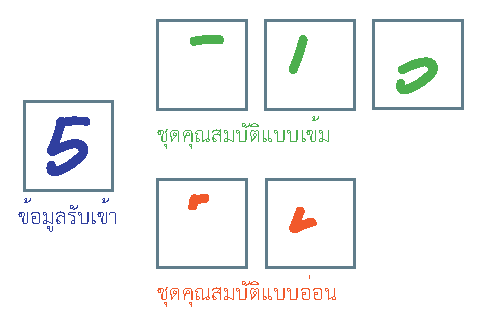
\includegraphics[width=\columnwidth]{images/strong-weak-features.pdf}
    \caption{ตัวอย่างชุดคุณสมบัติแบบอ่อน และแบบเข้มที่เป็นไปได้ จากเลข 5}
\end{figure*}

จะยกตัวอย่างกรณีการจำแนกเลข 5 เราอาจพิจารณาว่าเลข 5 ประกอบขึ้นจากขีดหนึ่งขีดแนวขวาง ขีดหนึ่งขีดแนวตั้ง และส่วนโค้งคล้ายวงกลม 

\subsection{การทดลองหาสัญญาณรบกวนบนชุดข้อมูล MNIST}

\subsection{การจำแนกกลุ่มของสัญญาณรบกวน}

\section{ผลลัพธ์}

\section{อภิปรายผล}

\section{สรุป}
\end{document}